% Portfolio Maker Pro - LaTeX Beamer Presentation
\documentclass[aspectratio=169]{beamer}

% Modern Theme
\usetheme{Madrid}
\usecolortheme{default}

% Custom Colors - Modern Purple/Blue Gradient Theme
\definecolor{primaryPurple}{RGB}{102, 126, 234}
\definecolor{secondaryPurple}{RGB}{118, 75, 162}
\definecolor{accentGreen}{RGB}{40, 167, 69}
\definecolor{darkText}{RGB}{51, 51, 51}
\definecolor{lightBg}{RGB}{248, 249, 250}

% Apply custom colors to theme
\setbeamercolor{palette primary}{bg=primaryPurple,fg=white}
\setbeamercolor{palette secondary}{bg=secondaryPurple,fg=white}
\setbeamercolor{palette tertiary}{bg=primaryPurple,fg=white}
\setbeamercolor{palette quaternary}{bg=secondaryPurple,fg=white}
\setbeamercolor{structure}{fg=primaryPurple}
\setbeamercolor{section in toc}{fg=primaryPurple}
\setbeamercolor{subsection in head/foot}{bg=secondaryPurple,fg=white}

% Custom block colors
\setbeamercolor{block title}{bg=primaryPurple,fg=white}
\setbeamercolor{block body}{bg=lightBg,fg=darkText}
\setbeamercolor{block title example}{bg=accentGreen,fg=white}
\setbeamercolor{block body example}{bg=lightBg,fg=darkText}

% Fonts
\usepackage{lmodern}
\usefonttheme{professionalfonts}
\usepackage{fontawesome5}

% Packages
\usepackage{tikz}
\usepackage{tcolorbox}
\usepackage{multicol}
\usepackage{graphicx}

% Remove navigation symbols
\setbeamertemplate{navigation symbols}{}

% Custom title page
\setbeamertemplate{title page}{
  \begin{tikzpicture}[remember picture,overlay]
    \fill[primaryPurple] (current page.south west) rectangle (current page.north east);
    \node[text=white,text width=0.8\paperwidth,align=center] at (current page.center) {
      {\Huge\textbf{\inserttitle}}\\[0.5cm]
      {\Large\insertsubtitle}\\[1cm]
      {\large\insertauthor}\\[0.3cm]
      {\small\insertdate}
    };
  \end{tikzpicture}
}

% Footer
\setbeamertemplate{footline}{
  \leavevmode%
  \hbox{%
  \begin{beamercolorbox}[wd=.5\paperwidth,ht=2.5ex,dp=1ex,left,leftskip=1em]{author in head/foot}%
    \usebeamerfont{author in head/foot}\insertshortauthor
  \end{beamercolorbox}%
  \begin{beamercolorbox}[wd=.5\paperwidth,ht=2.5ex,dp=1ex,right,rightskip=1em]{title in head/foot}%
    \usebeamerfont{title in head/foot}\insertframenumber{} / \inserttotalframenumber
  \end{beamercolorbox}}%
  \vskip0pt%
}

% Title Information
\title{Portfolio Maker Pro}
\subtitle{3D Portfolio Constructor Platform}
\author{Modern Web Development Project}
\date{November 2025}
\institute{Build stunning portfolios • No coding required • Professional results}

%----------------------------------------------------------------------------------------
\begin{document}

%----------------------------------------------------------------------------------------
% TITLE SLIDE
%----------------------------------------------------------------------------------------
\begin{frame}[plain]
  \titlepage
\end{frame}

%----------------------------------------------------------------------------------------
% SLIDE 2: PROJECT OVERVIEW
%----------------------------------------------------------------------------------------
\begin{frame}{Project Overview}
  \begin{columns}[T]
    \begin{column}{0.48\textwidth}
      \begin{block}{What is Portfolio Maker Pro?}
        A modern, feature-rich \textbf{web-based portfolio builder} that enables students, professionals, and creatives to design stunning portfolio websites \textcolor{accentGreen}{\textbf{without writing code}}.
        
        \vspace{0.3cm}
        Features:
        \begin{itemize}
          \item \faCheck\ Real-time preview
          \item \faCheck\ Multilingual support (4 languages)
          \item \faCheck\ 3D visual effects
          \item \faCheck\ Cloud-based storage
        \end{itemize}
      \end{block}
    \end{column}
    
    \begin{column}{0.48\textwidth}
      \begin{exampleblock}{Target Audience}
        \begin{itemize}
          \item \faGraduationCap\ \textbf{Students:} Showcase academic projects
          \item \faLaptopCode\ \textbf{Developers:} Display coding portfolio
          \item \faPaintBrush\ \textbf{Designers:} Present creative work
          \item \faBriefcase\ \textbf{Freelancers:} Professional portfolios
          \item \faUserTie\ \textbf{Job Seekers:} Stand out in job markets
        \end{itemize}
      \end{exampleblock}
    \end{column}
  \end{columns}
\end{frame}

%----------------------------------------------------------------------------------------
% SLIDE 3: KEY FEATURES
%----------------------------------------------------------------------------------------
\begin{frame}{Key Features}
  \begin{multicols}{2}
    \begin{tcolorbox}[colback=lightBg,colframe=primaryPurple,title=\faPalette\ Visual Editor]
      Drag-and-drop interface with real-time preview. See changes instantly.
    \end{tcolorbox}
    
    \begin{tcolorbox}[colback=lightBg,colframe=primaryPurple,title=\faGlobe\ Multilingual]
      Create portfolios in 4 languages: English, Ukrainian, Russian, Polish.
    \end{tcolorbox}
    
    \begin{tcolorbox}[colback=lightBg,colframe=primaryPurple,title=\faMobileAlt\ Responsive]
      Preview for desktop, tablet, and mobile. Looks great everywhere.
    \end{tcolorbox}
    
    \begin{tcolorbox}[colback=lightBg,colframe=primaryPurple,title=\faCube\ 3D Effects]
      Three.js integration for stunning visual effects in hero sections.
    \end{tcolorbox}
    
    \begin{tcolorbox}[colback=lightBg,colframe=primaryPurple,title=\faCloud\ Cloud Storage]
      Projects saved to Strapi backend. Access from anywhere.
    \end{tcolorbox}
    
    \begin{tcolorbox}[colback=lightBg,colframe=primaryPurple,title=\faImage\ Media Manager]
      Upload images with automatic optimization and validation.
    \end{tcolorbox}
    
    \begin{tcolorbox}[colback=lightBg,colframe=primaryPurple,title=\faBolt\ Auto-Save]
      Changes saved automatically every 500ms. Never lose work.
    \end{tcolorbox}
    
    \begin{tcolorbox}[colback=lightBg,colframe=primaryPurple,title=\faLayerGroup\ Section Library]
      Pre-built sections: Hero, About, Skills, Projects, Contact.
    \end{tcolorbox}
  \end{multicols}
\end{frame}

%----------------------------------------------------------------------------------------
% SLIDE 4: BENEFITS FOR STUDENTS
%----------------------------------------------------------------------------------------
\begin{frame}{Benefits for Students}
  \begin{exampleblock}{\faGraduationCap\ Showcase Academic Projects}
    Display coursework, research papers, and group projects with rich media. Add descriptions, tags, and links to GitHub repositories.
  \end{exampleblock}
  
  \begin{exampleblock}{\faBriefcase\ Career Preparation}
    Build professional online presence before graduation. Stand out in internship and job applications.
  \end{exampleblock}
  
  \begin{exampleblock}{\faRocket\ No Technical Barriers}
    Focus on content and design, not coding. No HTML, CSS, or JavaScript knowledge required.
  \end{exampleblock}
  
  \begin{exampleblock}{\faMoneyBillWave\ Free to Use}
    Open-source project with no subscription fees. Self-host or use free tier. Perfect for students on budget.
  \end{exampleblock}
  
  \begin{exampleblock}{\faBook\ Learn by Doing}
    Explore modern web technologies through user-friendly interface. Understand React, APIs, and responsive design.
  \end{exampleblock}
\end{frame}

%----------------------------------------------------------------------------------------
% SLIDE 5: BENEFITS FOR PROFESSIONALS
%----------------------------------------------------------------------------------------
\begin{frame}{Benefits for Professionals}
  \begin{block}{\faBolt\ Rapid Deployment}
    Create and launch professional portfolios in minutes, not days. Perfect for freelancers.
  \end{block}
  
  \begin{block}{\faSlidersH\ Complete Control}
    Customize every aspect without coding. Choose layouts, add content, manage multiple projects.
  \end{block}
  
  \begin{block}{\faChartLine\ Project Management}
    Organize multiple portfolio versions. Archive old projects, create new ones seamlessly.
  \end{block}
  
  \begin{block}{\faCodeBranch\ Version Control}
    Conflict detection prevents data loss when editing from multiple devices.
  \end{block}
  
  \begin{block}{\faGlobeAmericas\ Global Reach}
    Multilingual support for international markets. Create separate language versions easily.
  \end{block}
\end{frame}

%----------------------------------------------------------------------------------------
% SLIDE 6: TECHNICAL ARCHITECTURE
%----------------------------------------------------------------------------------------
\begin{frame}{Technical Architecture}
  \begin{block}{Modern Tech Stack}
    \begin{center}
      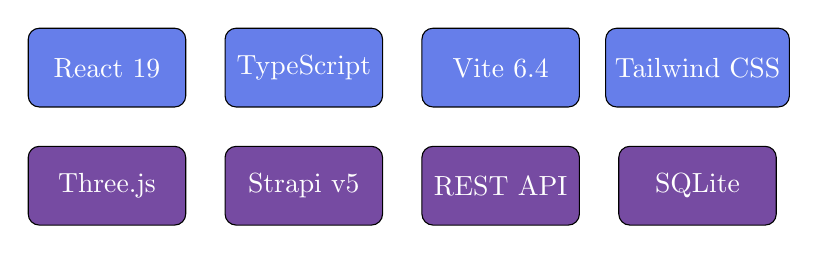
\begin{tikzpicture}
        \node[draw,rounded corners,fill=primaryPurple,text=white,minimum width=2cm,minimum height=1cm] at (0,0) {React 19};
        \node[draw,rounded corners,fill=primaryPurple,text=white,minimum width=2cm,minimum height=1cm] at (2.5,0) {TypeScript};
        \node[draw,rounded corners,fill=primaryPurple,text=white,minimum width=2cm,minimum height=1cm] at (5,0) {Vite 6.4};
        \node[draw,rounded corners,fill=primaryPurple,text=white,minimum width=2cm,minimum height=1cm] at (7.5,0) {Tailwind CSS};
        \node[draw,rounded corners,fill=secondaryPurple,text=white,minimum width=2cm,minimum height=1cm] at (0,-1.5) {Three.js};
        \node[draw,rounded corners,fill=secondaryPurple,text=white,minimum width=2cm,minimum height=1cm] at (2.5,-1.5) {Strapi v5};
        \node[draw,rounded corners,fill=secondaryPurple,text=white,minimum width=2cm,minimum height=1cm] at (5,-1.5) {REST API};
        \node[draw,rounded corners,fill=secondaryPurple,text=white,minimum width=2cm,minimum height=1cm] at (7.5,-1.5) {SQLite};
      \end{tikzpicture}
    \end{center}
  \end{block}
  
  \vspace{0.3cm}
  
  \begin{columns}[T]
    \begin{column}{0.48\textwidth}
      \textbf{\textcolor{primaryPurple}{Frontend Features:}}
      \begin{itemize}
        \item Component-based architecture
        \item State management (useReducer)
        \item Schema-driven dynamic forms
        \item Debounced autosave system
      \end{itemize}
    \end{column}
    
    \begin{column}{0.48\textwidth}
      \textbf{\textcolor{primaryPurple}{Backend Features:}}
      \begin{itemize}
        \item JWT authentication
        \item RESTful API integration
        \item Client-side routing
        \item Real-time preview rendering
      \end{itemize}
    \end{column}
  \end{columns}
\end{frame}

%----------------------------------------------------------------------------------------
% SLIDE 7: IMPLEMENTATION HIGHLIGHTS
%----------------------------------------------------------------------------------------
\begin{frame}{Implementation Highlights}
  \begin{multicols}{2}
    \begin{tcolorbox}[colback=lightBg,colframe=accentGreen,title=\faLock\ Authentication]
      Secure JWT-based login and registration. Protected routes.
    \end{tcolorbox}
    
    \begin{tcolorbox}[colback=lightBg,colframe=accentGreen,title=\faFolder\ Dashboard]
      Professional project management with CRUD operations.
    \end{tcolorbox}
    
    \begin{tcolorbox}[colback=lightBg,colframe=accentGreen,title=\faDatabase\ Persistent Storage]
      Full Strapi backend integration with auto-sync.
    \end{tcolorbox}
    
    \begin{tcolorbox}[colback=lightBg,colframe=accentGreen,title=\faSave\ Auto-Save]
      Intelligent debounced save with retry logic.
    \end{tcolorbox}
    
    \begin{tcolorbox}[colback=lightBg,colframe=accentGreen,title=\faFileImage\ Image Upload]
      Direct upload to Strapi with validation (5MB limit).
    \end{tcolorbox}
    
    \begin{tcolorbox}[colback=lightBg,colframe=accentGreen,title=\faWpforms\ Schema Forms]
      Dynamic field rendering based on JSON schemas.
    \end{tcolorbox}
    
    \begin{tcolorbox}[colback=lightBg,colframe=accentGreen,title=\faExclamationTriangle\ Conflict Detection]
      Timestamp-based version conflict detection.
    \end{tcolorbox}
    
    \begin{tcolorbox}[colback=lightBg,colframe=accentGreen,title=\faShieldAlt\ Access Control]
      Lifecycle hooks filter projects by owner.
    \end{tcolorbox}
  \end{multicols}
\end{frame}

%----------------------------------------------------------------------------------------
% SLIDE 8: PROJECT STATISTICS
%----------------------------------------------------------------------------------------
\begin{frame}{Project Statistics \& Scope}
  \begin{center}
    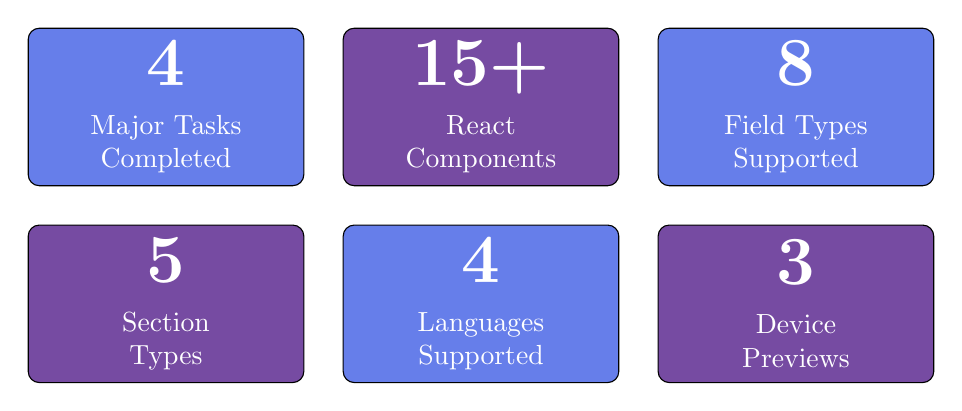
\begin{tikzpicture}
      % Stats boxes
      \node[draw,rounded corners,fill=primaryPurple,text=white,minimum width=3.5cm,minimum height=2cm,align=center] at (0,0) {
        \Huge\textbf{4}\\[0.2cm]
        \normalsize Major Tasks\\Completed
      };
      \node[draw,rounded corners,fill=secondaryPurple,text=white,minimum width=3.5cm,minimum height=2cm,align=center] at (4,0) {
        \Huge\textbf{15+}\\[0.2cm]
        \normalsize React\\Components
      };
      \node[draw,rounded corners,fill=primaryPurple,text=white,minimum width=3.5cm,minimum height=2cm,align=center] at (8,0) {
        \Huge\textbf{8}\\[0.2cm]
        \normalsize Field Types\\Supported
      };
      
      \node[draw,rounded corners,fill=secondaryPurple,text=white,minimum width=3.5cm,minimum height=2cm,align=center] at (0,-2.5) {
        \Huge\textbf{5}\\[0.2cm]
        \normalsize Section\\Types
      };
      \node[draw,rounded corners,fill=primaryPurple,text=white,minimum width=3.5cm,minimum height=2cm,align=center] at (4,-2.5) {
        \Huge\textbf{4}\\[0.2cm]
        \normalsize Languages\\Supported
      };
      \node[draw,rounded corners,fill=secondaryPurple,text=white,minimum width=3.5cm,minimum height=2cm,align=center] at (8,-2.5) {
        \Huge\textbf{3}\\[0.2cm]
        \normalsize Device\\Previews
      };
    \end{tikzpicture}
  \end{center}
\end{frame}

%----------------------------------------------------------------------------------------
% SLIDE 9: USE CASES
%----------------------------------------------------------------------------------------
\begin{frame}{Real-World Use Cases}
  \begin{columns}[T]
    \begin{column}{0.48\textwidth}
      \begin{alertblock}{\faLaptopCode\ Software Developer}
        \small
        \textbf{Scenario:} Recent graduate needs portfolio for job interviews.\\
        \textbf{Solution:} Creates portfolio with GitHub links, project descriptions in multiple languages.
      \end{alertblock}
      
      \begin{alertblock}{\faPaintBrush\ Graphic Designer}
        \small
        \textbf{Scenario:} Freelancer wants professional portfolio.\\
        \textbf{Solution:} Uses image upload for thumbnails, organizes work by categories with tags.
      \end{alertblock}
      
      \begin{alertblock}{\faGraduationCap\ University Student}
        \small
        \textbf{Scenario:} CS student applying for internships.\\
        \textbf{Solution:} Documents semester projects with tech stacks and demo links.
      \end{alertblock}
    \end{column}
    
    \begin{column}{0.48\textwidth}
      \begin{alertblock}{\faPenNib\ Content Writer}
        \small
        \textbf{Scenario:} Writer needs English and Russian portfolio.\\
        \textbf{Solution:} Uses multilingual support for both languages with article links.
      \end{alertblock}
      
      \begin{alertblock}{\faRocket\ Startup Founder}
        \small
        \textbf{Scenario:} Entrepreneur wants product landing page.\\
        \textbf{Solution:} Builds single-page portfolio with features and testimonials.
      \end{alertblock}
      
      \begin{alertblock}{\faChartBar\ Marketing Specialist}
        \small
        \textbf{Scenario:} Marketer displays campaign results.\\
        \textbf{Solution:} Creates data-driven portfolio with metrics and screenshots.
      \end{alertblock}
    \end{column}
  \end{columns}
\end{frame}

%----------------------------------------------------------------------------------------
% SLIDE 10: CONCLUSION
%----------------------------------------------------------------------------------------
\begin{frame}[plain]
  \begin{tikzpicture}[remember picture,overlay]
    \fill[primaryPurple] (current page.south west) rectangle (current page.north east);
    \node[text=white,text width=0.8\paperwidth,align=center] at (current page.center) {
      {\Huge\textbf{Why Portfolio Maker Pro?}}\\[1cm]
      
      \begin{minipage}{0.7\paperwidth}
        \Large
        \faCheck\ \textbf{Easy to Use:} No coding required, intuitive interface\\[0.4cm]
        \faCheck\ \textbf{Feature-Rich:} Everything you need in one platform\\[0.4cm]
        \faCheck\ \textbf{Professional Results:} Stunning portfolios that impress\\[0.4cm]
        \faCheck\ \textbf{Always Accessible:} Cloud-based, work from anywhere\\[0.4cm]
        \faCheck\ \textbf{Open Source:} Free to use, customize, and extend\\[1cm]
        
        \huge\textbf{Start building your portfolio today!}
      \end{minipage}
    };
  \end{tikzpicture}
\end{frame}

%----------------------------------------------------------------------------------------
\end{document}
